\documentclass{article}

\usepackage{stmaryrd}
\usepackage{amssymb}
\usepackage{tikz}
\usetikzlibrary{positioning, shadows}

\title{Interaction Diagram - Search By Series Extension 1A}
\author{Adam Hammes}

% no page number at bottom
\pagenumbering{gobble}

\begin{document}
\maketitle

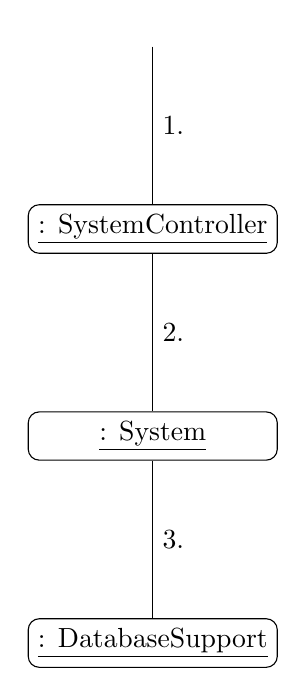
\begin{tikzpicture}[
  auto,
  block/.style = {
    minimum width = 9em,
    rectangle,
    draw=black,
    align=center,
    rounded corners
  },
  multiple/.style = {
    rectangle, draw, rounded corners, fill= white, 
    text width=9em, align= center,
    copy shadow = {
      ,fill=white, draw=black,
      shadow xshift=0.5mm, shadow yshift=-0.5mm
    }
  }
]

\node[] (start)  {};

\node[block, below = 2cm of start]      (controller) {\underline{: SystemController}};
\node[block, below = 2cm of controller] (system)     {\underline{: System}}; 
\node[block, below = 2cm of system]     (database)   {\underline{: DatabaseSupport}};

\draw (start) -- (controller) node[midway] {1.};
\draw (controller) -- (system) node[midway] {2.};
\draw (system) -- (database) node[midway] {3.};

\end{tikzpicture}

\vspace{0.5cm}

\begin{enumerate}
  \item \texttt{l:=searchBySeries(bid:String, sid:String):null}
  \item \texttt{l:=searchBySeries(bid:String, sid:String):null}
  \item \texttt{series:=getSeries(sid:String):null}
\end{enumerate}

\end{document}
